\chapter{Karp-Rabin Algorithm}

From Fundamental Theorem of Algebra (Theorem~\ref{thm:fundamental-algebra}), we see that every non-constant degree-$d$ polynomial:

\begin{itemize}
	\item can be factored
	\item has at most $d$ roots
	\item can be reconstructed from $d+1$ evaluations
\end{itemize}

However, for polynomials over integers in $\mathbb Z_p$ (a.k.a. $\mod p$), where $p$ is a prime, Theorem~\ref{thm:fundamental-algebra} does not hold (for example, $x^2+1 \mod 3$ has no root.)

Still, the last two properties hold for polynomials over $\mathbb Z_p$, i.e. it has at most $d$ roots and can be reconstructed from $d+1$ evaluations. This is the key observation for Karp-Rabin algorithm.

\section{Equality Testing}

\begin{problem}
Alice and Bob each have a string of length $n$ with alphabet $\Sigma$, and they want to determine if their strings are the same. They can only communicate by sending bits to each other, and they want to minimize the number of bits sent. How can they do this efficiently?
\end{problem}

A naive solution is to send the entire string, which requires $O(n)$ bits (very large).

\begin{lemma}
	The naive solution is optimal for deterministic algorithms, i.e. any deterministic algorithm must send $\Omega(n)$ bits in the worst case.
\end{lemma}
\begin{proof}
	If there's a deterministic algorithm that sends $o(n)$ bits, then there are at most $2^{o(n)}$ possible messages. Since there are $2^n$ possible strings, by the pigeonhole principle, there must be at least two different strings that produce the same message. Therefore, the algorithm cannot distinguish between these two strings, leading to a contradiction.
\end{proof}

Therefore, we need to use randomness to achieve better communication complexity. Note that it's sufficient to have an algorithm that accepts with certainty when the strings are equal, and rejects with probability $1/2$ when the strings are different. We can repeat the algorithm multiple times to reduce the error probability.

\begin{algorithm}[H]
	Alice and Bob agree on a prime $p>\max\{|\Sigma|, 2n\}$ and a random integer $x \in [p]$\;
	Alice computes $A(x) = \sum_{i=0}^{n-1} A[i] x^i \mod p$ and sends $A(x)$ to Bob\;
	Bob computes $B(x) = \sum_{i=0}^{n-1} B[i] x^i \mod p$\;
	Bob compares $A(x)$ and $B(x)$, accept if they are equal, and reject otherwise\;
	\caption{Karp-Rabin Algorithm for Equality Testing} \label{alg:karp-rabin-equality}
\end{algorithm}

\begin{theorem}
	Algorithm~\ref{alg:karp-rabin-equality} is correct, i.e. it accepts with certainty when the strings are equal, and rejects with probability at least $1/2$ when the strings are different.
\end{theorem}
\begin{proof}
	Suppose $A$ and $B$ are different, then $A(x) - B(x)$ is a non-zero polynomial of degree at most $n-1$. Since a non-zero polynomial of degree at most $n-1$ can have at most $n-1$ roots, the probability that $A(x) = B(x)$ (i.e. $A(x) - B(x) = 0$) is at most $\frac{n-1}{p} < \frac{1}{2}$.
\end{proof}

With a message size of $O(\log p) = O(\log n)$, Algorithm~\ref{alg:karp-rabin-equality} achieves a communication complexity of $O(\log n)$, which is exponentially better than the deterministic lower bound of $\Omega(n)$.

\section{String Matching}

\begin{problem}
Given a text string $T$ of length $n$ and a pattern string $P$ of length $m$ ($m<n$), determine if $P$ is a substring of $T$.
\end{problem}

Intuitively, we can apply equality testing to each substring of $T$ of length $m$, which leads to a time complexity of $O(nm)$. Our target here is to achieve a time complexity of $O(n)$.

Note that instead of computing the hash value of each substring from scratch, we can use the following rolling hash formula to compute the hash value of the next substring in $O(1)$ time:

\begin{align*}
	H[i]   & = \sum_{k=0}^{m-1} T[i+k] x^{m-1-k} \mod p \\
	H[i+1] & = (H[i] - T[i] x^{m-1}) x + T[i+m] \mod p
\end{align*}

\begin{note}
	This is different from the hash formula in Algorithm~\ref{alg:karp-rabin-equality} in that it reverses the order of coefficients,	because it's easier to compute the next hash value using the new one.
\end{note}

\begin{algorithm}[H]
	Fix a prime $p$ and a random $x \in [p]$\;
	Define $\text{PolyEval} (a_{m-1},\cdots,a_0) = a_{m-1}x^{m-1} + \cdots + a_0 \mod p$\;
	$H[0] \gets \text{PolyEval} (T[0],\cdots,T[m-1])$\;
	\For{$i \gets 1$ \KwTo $n-m$}{
		$H[i] \gets (H[i-1] - T[i-1] x^{m-1}) x + T[i+m-1] \mod p$\;
	}
	$h \gets \text{PolyEval} (P[0],\cdots,P[m-1])$\;
	List all occurrences of $h$ in $H$\;
	\For{each occurrence $i$}{
		\If{$T[i..i+m-1] = P$}{
			\Return True\;
		}
	}
	\Return False\;
	\caption{Karp-Rabin Algorithm for String Matching} \label{alg:karp-rabin-string-matching}
\end{algorithm}

\begin{theorem}
	The expected time complexity of Algorithm~\ref{alg:karp-rabin-string-matching} can be made $O(n + m\cdot \text{occ})$, where $\text{occ}$ is the number of occurrences of $P$ in $T$, by choosing a sufficiently large prime $p$.
\end{theorem}
\begin{proof}
	Let $Z$ be the number of false positives. We define indicator random variables $Z_i$ to be $1$ if there's a false positive at position $i$, and $0$ otherwise. The expected value of $Z_i$ is $\frac{m-1}{p}$, so from linearity of expectation:
	\[
		Z = \sum_{i=0}^{n-m} Z_i \implies \E[Z] = \sum_{i=0}^{n-m} \E[Z_i] = (n-m+1) \cdot \frac{m-1}{p} < \frac{n m}{p}
	\]
	Therefore, the expected time complexity of the algorithm is $O(n + m\cdot (\text{occ} + Z)) = O(n + m\cdot (\text{occ} + \frac{n m}{p}))$. By choosing $p>m^2$, we can make the expected time complexity $O(n + m\cdot \text{occ})$.
\end{proof}

If we don't want to see randomness in time complexity, we can just skip the checks and return true if there's a hash match.
In this case, the algorithm runs in $O(n)$ time, but it may return false positives with probability at most $\frac{n m}{p}$, which can be made arbitrarily small by choosing a sufficiently large prime $p$.

We claim here without proof:

\begin{theorem}
	The expected time complexity of Algorithm~\ref{alg:karp-rabin-string-matching}                   without checking hash collisions is $O(n)$, and the probability of returning a false positive is at most $\frac{1}{n}$ when $p \gg (n m)^2$.
\end{theorem}

\begin{definition}[Monte Carlo Algorithm and Las Vegas Algorithm]
	A \textbf{Monte Carlo algorithm} is a randomized algorithm that always runs in the stated time, but may return an incorrect answer with some probability. A \textbf{Las Vegas algorithm} is a randomized algorithm that always returns the correct answer, but may run in a random amount of time.

	For example, Algorithm~\ref{alg:karp-rabin-string-matching} with checks is a Las Vegas algorithm, while Algorithm~\ref{alg:karp-rabin-string-matching} without checks is a Monte Carlo algorithm.
\end{definition}

\section{Examples Using Karp-Rabin Algorithm}

\begin{question}[2-D Pattern Matching]
	Given a 2-D text matrix $T$ of size $n\times n$ and a 2-D pattern matrix $P$ of size $m\times m$ ($m<n$), determine if $P$ is a submatrix of $T$.
\end{question}

A common approach for a multi-dimensional problem is to reduce it to a one-dimensional problem. We can compute the hash value of each row of $T$ and $P$ using the same method as in Algorithm~\ref{alg:karp-rabin-string-matching}, and then apply the Karp-Rabin algorithm for string matching on the resulting hash values.

\begin{align*}
	H_0 [i,j] & = \sum_{k=0}^{m-1} T[i+k][j] x^{m-1-k} \mod p    \\
	H[i,j]    & = \sum_{k=0}^{m-1} H_0 [i][j+k] x^{m-1-k} \mod p
\end{align*}

The rest of the algorithm is omitted here.

\begin{question}[Longest Common Substring]
	Given two strings $A$ and $B$, find the longest common substring of $A$ and $B$.
\end{question}

See homework 3.

\chapter {K.M.P. Algorithm and Finite Automata}

\begin{definition}[Finite Automaton]
	A \textbf{finite automaton} is a mathematical model of computation that consists of a finite set of states, a set of input symbols, a transition function that maps pairs of states and input symbols to states, an initial state, and a set of accepting states. It can be used to recognize patterns in strings and is often represented as a directed graph.
\end{definition}

Finite automata can be used to solve the string matching problem by constructing an automaton that recognizes the pattern string $P$ and then running the automaton on the text string $T$ in $O(n)$ time with no randomness involved.

As this is not a topic of this course, we will only show an example here.

This is a finite automaton for the pattern string ``abcab'' (one may find it very familiar if he has taken EECS 370):

\begin{center}
	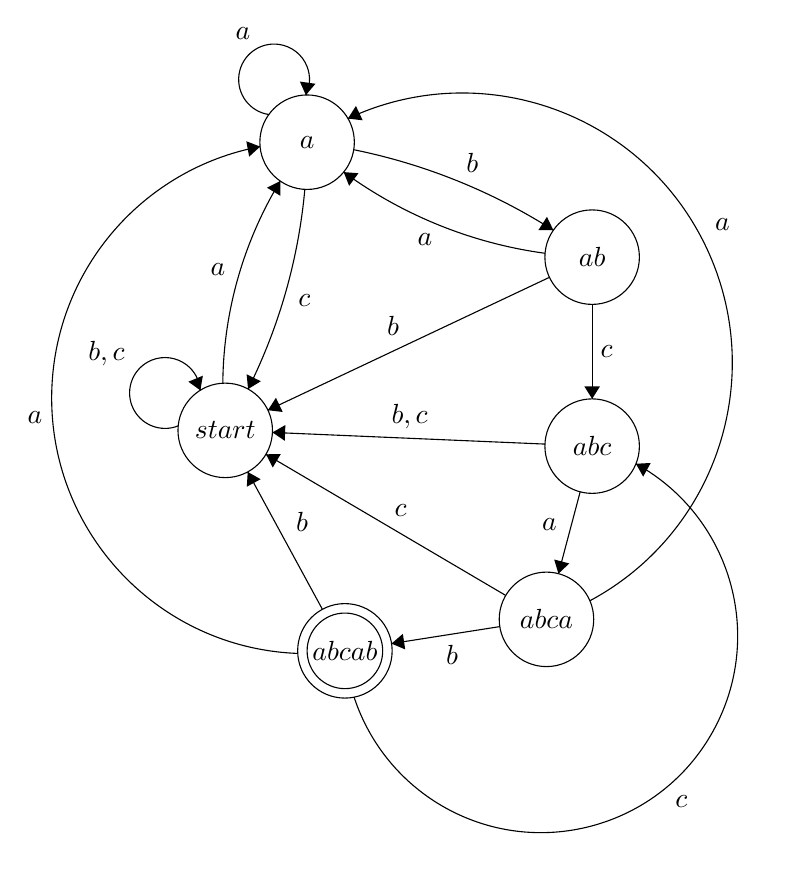
\begin{tikzpicture}[scale=0.2]
		\tikzstyle{every node}+=[inner sep=0pt]
		\draw [black] (15.2,-27.4) circle (3);
		\draw (15.2,-27.4) node {$start$};
		\draw [black] (20.4,-9.1) circle (3);
		\draw (20.4,-9.1) node {$a$};
		\draw [black] (38.5,-16.4) circle (3);
		\draw (38.5,-16.4) node {$ab$};
		\draw [black] (38.5,-28.4) circle (3);
		\draw (38.5,-28.4) node {$abc$};
		\draw [black] (35.6,-39.4) circle (3);
		\draw (35.6,-39.4) node {$abca$};
		\draw [black] (22.8,-41.4) circle (3);
		\draw (22.8,-41.4) node {$abcab$};
		\draw [black] (22.8,-41.4) circle (2.4);
		\draw [black] (15.047,-24.406) arc (-180.48683:-211.23849:25.17);
		\fill [black] (18.7,-11.57) -- (17.85,-11.99) -- (18.71,-12.51);
		\draw (15.24,-17.18) node [left] {$a$};
		\draw [black] (12.226,-27.109) arc (292.1427:4.1427:2.25);
		\draw (8.84,-22.55) node [left] {$b,c$};
		\fill [black] (13.62,-24.86) -- (13.78,-23.93) -- (12.86,-24.31);
		\draw [black] (23.361,-9.578) arc (78.53832:57.53177:37.487);
		\fill [black] (36.04,-14.69) -- (35.63,-13.84) -- (35.09,-14.68);
		\draw (30.89,-11.03) node [above] {$b$};
		\draw [black] (38.5,-19.4) -- (38.5,-25.4);
		\fill [black] (38.5,-25.4) -- (39,-24.6) -- (38,-24.6);
		\draw (39,-22.4) node [right] {$c$};
		\draw [black] (37.74,-31.3) -- (36.36,-36.5);
		\fill [black] (36.36,-36.5) -- (37.05,-35.85) -- (36.09,-35.6);
		\draw (36.29,-33.4) node [left] {$a$};
		\draw [black] (32.64,-39.86) -- (25.76,-40.94);
		\fill [black] (25.76,-40.94) -- (26.63,-41.31) -- (26.48,-40.32);
		\draw (29.6,-40.99) node [below] {$b$};
		\draw [black] (17.981,-7.345) arc (261.76333:-26.23667:2.25);
		\draw (16.32,-2.62) node [above] {$a$};
		\fill [black] (20.32,-6.11) -- (20.93,-5.39) -- (19.94,-5.25);
		\draw [black] (20.255,-12.096) arc (-5.18263:-26.54269:35.565);
		\fill [black] (16.65,-24.78) -- (17.46,-24.28) -- (16.56,-23.84);
		\draw (19.81,-19.16) node [right] {$c$};
		\draw [black] (35.79,-17.68) -- (17.91,-26.12);
		\fill [black] (17.91,-26.12) -- (18.85,-26.23) -- (18.42,-25.33);
		\draw (25.86,-21.39) node [above] {$b$};
		\draw [black] (35.511,-16.155) arc (-97.742:-126.18791:28.064);
		\fill [black] (22.72,-11) -- (23.07,-11.87) -- (23.66,-11.07);
		\draw (27.89,-14.89) node [below] {$a$};
		\draw [black] (35.5,-28.27) -- (18.2,-27.53);
		\fill [black] (18.2,-27.53) -- (18.98,-28.06) -- (19.02,-27.06);
		\draw (26.91,-27.33) node [above] {$b,c$};
		\draw [black] (41.276,-29.519) arc (61.15465:-161.90341:12.487);
		\fill [black] (41.28,-29.52) -- (41.74,-30.34) -- (42.22,-29.47);
		\draw (44.17,-50.57) node [below] {$c$};
		\draw [black] (19.809,-41.564) arc (-92.14601:-259.35506:16.238);
		\fill [black] (17.42,-9.38) -- (16.54,-9.04) -- (16.72,-10.02);
		\draw (3.62,-26.59) node [left] {$a$};
		\draw [black] (21.37,-38.76) -- (16.63,-30.04);
		\fill [black] (16.63,-30.04) -- (16.57,-30.98) -- (17.45,-30.5);
		\draw (19.67,-33.22) node [right] {$b$};
		\draw [black] (22.992,-7.597) arc (115.09839:-61.81711:17.137);
		\fill [black] (22.99,-7.6) -- (23.93,-7.71) -- (23.5,-6.8);
		\draw (46.27,-14.32) node [right] {$a$};
		\draw [black] (33.01,-37.88) -- (17.79,-28.92);
		\fill [black] (17.79,-28.92) -- (18.22,-29.76) -- (18.73,-28.9);
		\draw (26.34,-32.9) node [above] {$c$};
	\end{tikzpicture}
\end{center}

The ``accepting state'' here means that we need to record the position of the text string when we reach this state (as we complete a match), and then proceed to the next character.
